\documentclass[a4paper,oneside,12pt]{book}
% Package yang diperlukan
\usepackage{graphicx} \usepackage{titling} \usepackage{geometry} \usepackage{listings}
\usepackage{xcolor} \usepackage{float} \usepackage{hyperref} \usepackage{indentfirst}
\usepackage{url} \usepackage{fancyhdr} \newcommand{\customfbox}[2]{%
  \setlength{\fboxsep}{0pt}%
  \setlength{\fboxrule}{0.5pt}
  \fcolorbox{black}{white}{#2}
}

% Pengaturan margin umum untuk isi laporan
\geometry{left=3cm, right=2.5cm, top=2cm, bottom=2.5cm}

% Pengaturan untuk kode
\definecolor{codegreen}{rgb}{0,0.6,0}
\definecolor{codegray}{rgb}{0.5,0.5,0.5}
\definecolor{codepurple}{rgb}{0.58,0,0.82}
\definecolor{backcolour}{rgb}{0.95,0.95,0.92}
\definecolor{darkblue}{rgb}{0,0,0.6}

% Common style untuk semua listing
\lstdefinestyle{commonstyle}{
    backgroundcolor=\color{backcolour}, 
    breakatwhitespace=false, 
    breaklines=true, 
    captionpos=b, 
    keepspaces=true,
    numbers=left, 
    numbersep=5pt, 
    showspaces=false, 
    showstringspaces=false,
    showtabs=false, 
    tabsize=2, 
    frame=single,
    basicstyle=\ttfamily\footnotesize,
    numberstyle=\tiny\color{codegray}
}

% Pengaturan untuk kode HTML
\lstdefinestyle{htmlstyle}{
    style=commonstyle,
    language=HTML,
    commentstyle=\color{codegreen},
    keywordstyle=\color{codepurple},
    stringstyle=\color{codegreen}
}

% Pengaturan untuk kode Python
\lstdefinestyle{pythonstyle}{
    style=commonstyle,
    language=Python,
    commentstyle=\color{codegreen},
    keywordstyle=\color{darkblue},
    stringstyle=\color{codepurple},
    emph={import,from,class,def,for,while,if,else,elif,try,except,finally},
    emphstyle=\color{darkblue}
}

% Pengaturan untuk kode SQL
\lstdefinestyle{sqlstyle}{
    style=commonstyle,
    language=SQL,
    commentstyle=\color{codegreen},
    keywordstyle=\color{darkblue},
    stringstyle=\color{codepurple},
    emph={SELECT,FROM,WHERE,INSERT,UPDATE,DELETE,CREATE,DROP},
    emphstyle=\color{darkblue}
}

% Pengaturan untuk kode JavaScript
\lstdefinestyle{javascriptstyle}{
    style=commonstyle,
    language=JavaScript,
    commentstyle=\color{codegreen},
    keywordstyle=\color{darkblue},
    stringstyle=\color{codepurple},
    emph={function,var,let,const,return,if,for,while,do,else,switch,case},
    emphstyle=\color{darkblue}
}

\lstdefinestyle{cssstyle}{
    style=commonstyle,
    language=CSS,
    commentstyle=\color{codegreen},
    keywordstyle=\color{darkblue},
    stringstyle=\color{codepurple},
    emph={color, background, font, margin, padding, border, display, position, width, height},
    emphstyle=\color{darkblue}
}

% Pengaturan untuk URL
\hypersetup{
    colorlinks=true, 
    linkcolor=black, 
    filecolor=black, 
    urlcolor=black,
    pdftitle={Laporan Praktikum}, 
    pdfpagemode=FullScreen, 
    breaklinks=true
}

% Pengaturan untuk nomor halaman di tengah bawah
\pagestyle{fancy}
\fancyhf{}
\fancyfoot[C]{\thepage}
\renewcommand{\headrulewidth}{0pt}

\fancypagestyle{plain}{
    \fancyhf{}
    \fancyfoot[C]{\thepage}
    \renewcommand{\headrulewidth}{0pt}
}

% Judul, Penulis, Tanggal
\title{Laporan Praktikum \\ Praktikum Struktur Data \\ Pertemuan 6 \\ Deque}
\date{2025-03-20}

% Penyesuaian nama Daftar Pustaka dan Daftar Isi
\renewcommand\bibname{Daftar Pustaka}
\renewcommand{\contentsname}{Daftar Isi}

\begin{document}

% Halaman Cover dengan margin khusus
\newgeometry{left=3cm, right=2.5cm, top=3cm, bottom=3cm}
\begin{titlingpage}
\begin{center}
\vspace{4cm}
\begin{huge}
\textbf{\thetitle} \\
\end{huge}
\vspace{1cm}
\includegraphics[height=9.5cm]{lambang ugm.png} \\
\vspace{1cm}
\begin{Large}
\textbf{Disusun oleh:} \\
\vspace{0.5cm}
Hafidz Rizqullah Prasetya \\
24/535493/SV/24243 \\
PL2A1 \\
\end{Large}
\vspace{1cm}
\begin{Large}
\textbf{Dosen Pengampu:} \\
\vspace{0.5cm}
Dr. Umar Taufiq, S.Kom., M.Cs. \\
\end{Large}
\vspace{1cm}
\thedate
\end{center}
\end{titlingpage}
\restoregeometry

% Daftar Isi
\tableofcontents
\newpage

\chapter*{Tujuan Praktikum}
\addcontentsline{toc}{chapter}{Tujuan Praktikum}
\begin{enumerate}
\item ini tujuan
\item ini tujuan
\item ini tujuan
\end{enumerate}

\chapter*{Dasar Teori}
\addcontentsline{toc}{chapter}{Dasar Teori}
\setcounter{chapter}{2}
\setcounter{section}{0}
\section{Pengenalan Deque}
Deque sering digunakan dalam berbagai aplikasi seperti:

\begin{itemize}

    \item \textbf{Pemrograman Kompetitif:} Untuk implementasi struktur data antrian yang efisien.


    \item \textbf{Simulasi:} Untuk memodelkan antrean yang memiliki proses masuk dan keluar di kedua ujung.


    \item \textbf{Algoritma Sliding Window:} Untuk mengoptimalkan pencarian nilai maksimum atau minimum dalam jendela yang bergerak.

\end{itemize}

\section{Bagian 2}
ssddadsad



\chapter*{Hasil dan Pembahasan}
\addcontentsline{toc}{chapter}{Hasil dan Pembahasan}
\setcounter{chapter}{3}
\setcounter{section}{0}
\section{Latihan 1}

\subsection{Soal 1}

\begin{lstlisting}[language=Python, style=pythonstyle]
Testing
\end{lstlisting}

\begin{figure}[H]
\centering
\customfbox{1pt}{
    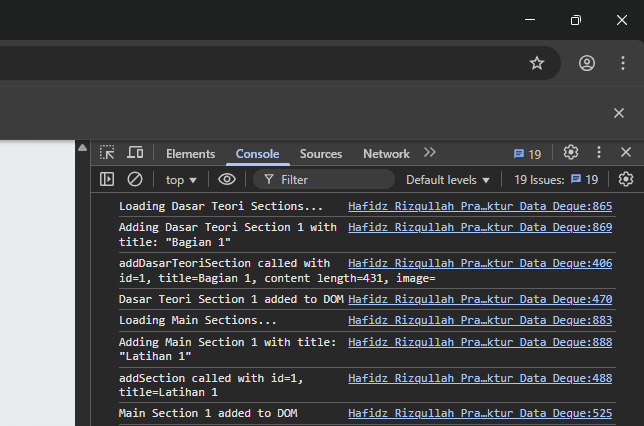
\includegraphics[width=0.78\textwidth, keepaspectratio]{img_20250327005619_3dea44.png}
}
\caption{Soal 1}
\label{fig:1_1}
\end{figure}

\textbf{Penjelasan:} Kode ini merupakan struktur HTML dasar dengan elemen \texttt{<ul>} berkelas \texttt{flex-container} yang berisi beberapa \texttt{<li>} berkelas \texttt{flex-item} (angka 1 hingga 6). 



Bagian \texttt{<head>} mencakup meta tag untuk karakter encoding, kompatibilitas browser, viewport, dan tautan ke file CSS eksternal (\texttt{style.css}). 



Kode CSS mendefinisikan \texttt{.flex-container} sebagai flexbox dengan arah baris yang dapat membungkus, distribusi ruang merata, tanpa padding/margin, dan menghapus gaya daftar bawaan. 



Sementara \texttt{.flex-item} memiliki latar belakang tomato, padding 5px, dimensi 200x150px, margin atas 10px, tinggi baris 150px, teks putih tebal dengan ukuran 3em, dan perataan tengah.



\chapter*{Kesimpulan}
\addcontentsline{toc}{chapter}{Kesimpulan}
\setcounter{chapter}{4}
\setcounter{section}{0}
Praktikum ini berfokus pada pembuatan tata letak responsif menggunakan HTML dan CSS dengan pendekatan Flexbox, termasuk menyelesaikan tantangan ``Article Preview Component'' dari Frontend Mentor. 



Saya mengakses Frontend Mentor, login menggunakan akun GitHub, dan memilih tantangan tersebut untuk membangun komponen artikel yang responsif.

\newpage
\addcontentsline{toc}{chapter}{Daftar Pustaka}
\begin{thebibliography}{99}
\begin{document}CSS Flexbox,'' w3schools.com, 2025. [Online]. \\
Available: \textbackslash\{\}url\{https://www.w3schools.com/css/css3\_flexbox.asp\}. [Accessed: 25-Mar-2025].
\end{thebibliography}

\end{document}
